\documentclass[11pt,a4paper]{article}
\usepackage[top=80px, left=70px, right=70px]{geometry}

\usepackage[T1]{fontenc}
\usepackage[utf8]{inputenc}
\usepackage{lmodern}
\usepackage[francais]{babel}
\usepackage{graphicx}
\usepackage{float}

\usepackage{algorithm}
\usepackage{algorithmic}
\usepackage{amssymb}
\usepackage{url}

\usepackage[table]{xcolor}


\renewcommand{\algorithmicrequire}{\textbf{Input:}}
\renewcommand{\algorithmicensure}{\textbf{Output:}}

\title{Comprendre Bitcoin\\
Rapport de projet INFRES357
}

\author{Pierre Galland, Benoît de Laitre}

\begin{document}
\maketitle

\tableofcontents
 \nocite{*}
 
\newpage

\section*{Introduction}

Bitcoin a fait beaucoup l'actualité durant ces deux dernières années mais la seule lecture d'articles de presse ne permet ni de comprendre de quoi il s'agit ni comment cela fonctionne. En effet, bien que n'utilisant que des techniques cryptographiques connues depuis assez longtemps, Bitcoin repose sur une architecture relativement complexe. Le but de ce rapport est de donner une idée suffisamment précise du fonctionnement général de Bitcoin. On n'entrera pas dans le détail des implémentations (en particulier on ne discutera pas des fonctions cryptographiques utilisées) mais on s'intéressera plutôt à l'architecture de Bitcoin. Les sections 1 et 2 expliquent le protocole en lui-même, tandis que la section 3 s'intéresse à l'écosystème qui doit être mis en place autour du protocole afin de le rendre utilisable, et les problématiques de sécurité associées.

\section{Les transactions Bitcoin}

\subsection{Briques de base}

Le protocole de Bitcoin utilise plusieurs briques de bases de la cryptographie : le chiffrement asymétrique, la signature et le hachage. C'est d'ailleurs là que réside l'intérêt de ce protocole, c'est un assemblage astucieux de briques qui existent depuis de nombreuses années et qui sont très bien connues, pourtant cet assemblage crée une technologie totalement nouvelle.

\subsubsection{Chiffrement asymétrique}

Le principe du chiffrement asymétrique est que les clefs vont par paire, une clef publique et une clef privé $(K_{Pub}, K_{Pri})$. On peut voir les clefs comme des suites finies de caractères ou de chiffres, et les message aussi. Il est possible de chiffrer un message avec la clef privé et alors le message chiffré ne pourra être déchiffré qu'avec la clef publique correspondante. De même on peut chiffrer un message avec la clef publique et alors il ne pourra être déchiffré qu'avec la clef privé correspondante. Considérons l'exemple classique de Bob et Alice, ils possède chacun une paire clef publique/clef privée. La paire de clefs de Bob est 
$(K_{Pub}^{B}, K_{Pri}^{B})$ et celle d'Alice est $(K_{Pub}^{A}, K_{Pri}^{A})$.\\\\

Si Bob veut envoyer un message $mess$ à Alice qu'elle seule pourra lire, alors il chiffre son message avec le clef publique d'Alice, et il obtient le message chiffré $*mess*$ :

$$chiffrer(mess, ~K_{Pub}^{A}) \rightarrow *mess*$$

Il envoie alors ce message $*mess*$ à Alice, qui quand elle le reçoit le déchiffre avec sa clef privée $K_{Pri}^{A}$ :

$$déchiffrer(*mess*, ~K_{Pri}^{A}) \rightarrow mess$$

Si Alice essayait de déchiffrer le message $*mess*$ avec une autre clef que sa clef privée $K_{Pri}^{A}$ alors cela ne marcherait pas, elle obtiendrait n'importe quoi (une suite de symbole qui n'a rien à voir avec le message $mess$). Donc comme on considère qu'Alice est la seule à connaître sa clef privée, elle est la seule à pouvoir déchiffrer le message.

$$déchiffrer(*mess*, ~K_{Pri}^{autre}) \rightarrow n'importe~quoi$$

On peut également utiliser la paire clef publique/clef privée dans l'autre sens. Si Bob chiffre un message avec sa clef privée $K_{Pri}^{B}$ alors on ne pourra le déchiffrer qu'avec sa clef publique $K_{Pub}^{B}$. En essayant de le déchiffrer avec une autre clef $K_{Pub}^{autre}$ on obtiendrait n'importe quoi.\\\\ Ainsi si Alice veut que Bob prouve qu'il est bien Bob donc qu'il connaît la clef privée $K_{Pri}^{B}$, sans qu'il ait à révéler cette clef, alors elle peut créer un message $mess2$ et demander à Bob de le chiffrer avec sa clef $K_{Pri}^{B}$ et de lui envoyer le résultat $*mess2*$. Alice va ensuite déchiffrer $*mess2*$ avec la clef publique de Bob $K_{Pub}^{B}$ et si elle retombe bien sur $mess2$ cela prouve que Bob est bien Bob (qu'il connaît la clef $K_{Pri}^{B}$). Ce mécanisme sera très utile pour la signature, décrite plus loin.
\subsubsection{Hachage cryptographique}

On considère toujours nos messages comme des suites finies de caractères ou de chiffres (d'ailleurs in fine sur un ordinateur toute donnée est une suite finie de chiffres). Le but d'une fonction de hachage cryptographique $h$ est de transformer chaque message de taille inférieure à $T$ (où $T$ est très très grand) en un message de taille beaucoup plus petite que $T$ (par exemple dans Bitcoin en message de longueur 256 chiffres). Si j'ai un message $mess$ assez long alors $h(mess)$ sera beaucoup plus petit que $mess$. On appellera $h(mess)$ le hash de $mess$. \\\\
Prenons un exemple avec la fonction de hachage SHA-256, qui est utilisée dans Bitcoin. Je considère le message $mess$ suivant et je calcule son $h(mess)$ : 
$$mess = Un~message~pas~très ~long, ~juste ~pour ~faire ~un ~exemple $$
$$h(mess) \rightarrow 6423e8584411fee28e5064799d8a230c64f999c448c769ab7d309baba9a33f42$$
Le but de la fonction de hachage est également que le hash d'un message puisse l'identifier de manière presque unique. Ainsi à priori si je considère deux messages différents alors leurs hashs sont également différents.  
$$mess1~ \neq ~mess2~ \Rightarrow ~presque~ toujours~ h(mess1)~ \neq ~h(mess2)$$
Un autre point important est que si je connais seulement le hash du message $h(mess)$ ainsi que la fonction de hachage $h$ mais que je ne connais pas le message $mess$ alors je ne puisse pas retrouver quel est le message $mess$. Il est impossible (cela demande trop de puissance de calcul) de retrouver le message à partir de son hash.
$$ h~ et ~h(mess) \nrightarrow mess$$
Enfin si je considère un message $mess1$ et ma fonction de hachage $h$, il m'est impossible (une fois encore cela demande trop de puissance de calcul) de trouver un message $mess2$ tel que $h(mess1) ~=~ h(mess2)$.\\\\
Les fonctions de hachage jouent un rôle très important dans le protocol Bitcoin !

\subsubsection{Signature}

Le but de la signature électronique est de s'assurer que le message que l'on reçoit a bien été envoyé par la personne qui signe, et que le message n'a pas été modifié entre le moment de la signature et sa réception. Reprenons l'exemple de Bob et Alice, avec leurs paires de clefs respectives $(K_{Pub}^{B}, K_{Pri}^{B})$ et $(K_{Pub}^{A}, K_{Pri}^{A})$. Pour qu'Alice puisse être certaine que le message qu'elle reçoit de Bob est bien de lui et qu'il n'a pas été modifié en cours de route il faut que Bob signe son message :\\

Après avoir écrit son message $mess$, Bob calcul son hash $h(mess)$

$$ mess ~ \rightarrow ~ h(mess) $$

Puis il utilise chiffre ce hash avec sa clef privée :

$$ chiffrer(h(mess),~ K_{Pri}^{B}) \rightarrow ~ *h(mess)* $$

Ce $*h(mess)*$ constitue la signature du message. Bob envoie à Alice le message avec sa signature : $ (mess, ~*h(mess)*)$. Lorsque Alice reçoit le message et la signature elle vérifie que la signature est valide et qu'elle provient bien de Bob.\\\\

Alice reçoit donc $(mess1,  ~*h(mess)*)$, on écrit $mess1$ car pour le moment on ne sait pas s'il s'agit bien du message original de Bob (il a peut-être été modifié par quelqu'un l'ayant intercepté). Alice calcule le hash de $mess1$ :

$$ mess1 ~ \rightarrow ~ h(mess1) $$

Puis elle déchiffre $*h(mess)*$ avec la clef publique de Bob. En le déchiffrant avec la clef publique de Bob $K_{Pub}^{B} $ elle s'assure que $*h(mess)*$ a bien été chiffré avec la clef privé de Bob $K_{Pri}^{B} $. En effet s'il avait été chiffré avec une autre clef privée alors en le déchiffrant avec $K_{Pub}^{B}$ on obtiendrait n'importe quoi. Comme à priori on n'est pas encore sûr que le $*h(mess)*$ que l'on déchiffre a bien été chiffré avec la clef privée de Bob, on note $?h(mess)?$ ce que l'on obtient :

$$ déchiffrer(*h(mess)*,~ K_{Pub}^{B})~ \rightarrow ~?h(mess)? $$

Enfin on compare $h(mess1)$ et $?h(mess)?$, s'ils sont égaux alors on est sûr (modulo la solidité de la fonction de hachage et de l'algorithme de chiffrement) que le message est bien de Bob et qu'il n'a pas été modifié, s'ils sont différents alors on ne peut pas faire confiance à ce message.\\\\
On peut se convaincre que c'est la cas en reprenant le processus et en imaginant qu'un attaquant modifie le message et/ou la signature en cours de route, ou qu'il essaie d'envoyer le message avec sa paire de clefs. On verra qu'à la fin le test que fait Alice donne bien $h(mess1) ~\neq~ ?h(mess)?$ (en gardant à l'esprit qu'Alice connaît la clef publique de Bob).\\
En revanche si un attaquant connaît la clef privée de Bob alors il peut très bien se faire passer pour lui !



\subsection{Une transaction Bitcoin}

\subsubsection{Identité et adresses}

Dans le protocole Bitcoin la notion d'identité repose sur le chiffrement asymétrique donc un individu est une paire clef publique/clef privée. Sachant que l'on peut générer la clef publique à partir de la clef privée, un individu est une clef privée. On parle ici d'individus dans le protocole, car une personne réelle peut très bien avoir plusieurs clefs privées et donc correspondre à plusieurs individus dans le protocole. C'est d'ailleurs normalement le cas. Chaque personne réelle possédant des bitcoins a au moins une centaine de clefs privées, donc correspond à de nombreux individus théoriques dans le protocole.\\
Les individus sont identifiés dans le protocole par leur adresse. Une adresse est un hash de clef publique. Par exemple 3J98t1WpEZ73CNmQviecrnyiWrnqRhWNLy est une adresse. Pour vérifier qu'une adresse $addr$ correspond bien à la clef publique $K_{Pub}$ on a juste à vérifier que $h(K_{Pub})~ ==~ addr$ où $h$ est la fonction de hachage définie par le protocole.

\subsubsection{Structure d'une transaction}

Tout d'abord on va considérer qu'il existe un "livre de compte" partagé entre tous les utilisateurs de Bitcoin et que chaque transaction valide est inscrite dans ce livre de compte de manière chronologique. On verra par la suite quel procédé permet l'existence de ce livre de compte, qu'on appelle la Blockchain.\\\\
Chacun peut donc accéder à l'historique de toutes les transactions valides qui ont été effectuées depuis la création de Bitcoin. Il est important de comprendre qu'il n'existe pas de pièce ou de billet de bitcoin, même virtuels. Il n'y a pas de fichiers qui représentent des bitcoins. C'est seulement la Blockchain (le livre de compte partagé) qui indique le nombre de bitcoins associé à chaque adresse.  Même cette vision n'est pas tout à fait exacte. La Blockchain n'est que l'historique de toutes les transactions valides effectuées. Il est donc plus correct de dire qu'on peut calculer le nombre de bitcoin de chaque adresse à partir de la Blockchain.\\\\
Prenons un exemple : on suppose que Bob veut envoyer 1 btc à Alice (on utilisera l'abréviation btc pour désigner l'unité de monnaie bitcoin). Bob et Alice ont toujours chacun une clef privée, respectivement $K_{Pri}^{B}$ et $K_{Pri}^{A}$, et ils ont également une adresse bitcoin : $adr_B = h(K_{Pub}^{B})$ et $adr_A = h(K_{Pub}^{A})$.\\\\
Pour que Bob puisse envoyer 1 btc, il faut qu'il dispose d'au moins 1 btc. Cela signifie qu'il faut qu'il existe dans la Blockchain une transaction qui envoie au moins 1 btc à l'adresse $adr_B$. Supposons que ce soit le cas, il y a dans la Blockchain une transaction $Tx_1$ qui envoie 1 btc à l'adresse  $adr_B$. Bob va donc retransférer vers Alice l'argent qu'il a reçu de $Tx_1$.
La transaction $Tx$ de Bob contient donc les éléments suivants :\\


\begin{figure}[H]
\begin{itemize}
\renewcommand{\labelitemi}{$\bullet$}
\renewcommand{\labelitemii}{$\star$}

\item Input
\begin{itemize}
\item $h(Tx_1)$
\item $K_{Pub}^{B}$
\item[$\bullet$] $signature(K_{Pri}^{B}, Tx^*)$
\end{itemize}

\item Output
\begin{itemize}
\item value : 1 btc
\item $adr_A$
\end{itemize}

\end{itemize}

\caption{Transaction $Tx$}
\end{figure}

\noindent La transaction contient donc 5 champs :\\\\
Dans la partie Input la transaction indique quelle transaction précédente est utilisée pour récupérer les bitcoins. Ici c'est la transaction $Tx_1$, c'est pour cela que le premier champ est $h(Tx_1)$. Le deuxième champ est la clef publique de Bob. En effet Bob veut utiliser les bitcoins donnés à $adr_B$ par $Tx_1$, il doit donc prouver qu'il possède bien l'adresse $adr_B$. Pour cela il fournit 
$K_{Pub}^{B}$ et $signature(K_{Pri}^{B}, Tx^*)$. On peut donc vérifier d'une part que $h(K_{Pub}^{B}) == adr_B$, donc que l'adresse $adr_B$ correspond bien à la clef $K_{Pub}^{B}$, et d'autre part que $signature(K_{Pri}^{B}, Tx^*)$ est valide, donc que celui qui émet le message possède bien la clef privée $K_{Pri}^{B}$. Ce qui est signé est $Tx^*$ c'est à dire la transaction $Tx$ sans la signature (les éléments précédés d'une étoile sur la figure).\\\\
Dans la partie Output Bob indique qu'il souhaite donner 1 btc (champ value) à l'adresse $adr_A$, soit à Alice.

\subsubsection{Sécurité de la transaction}

Une fois que Bob a écrit sa transaction, il la diffuse sur le réseau Bitcoin afin qu'elle soit intégrée dans la Blockchain et devienne ainsi une transaction valide, faisant partie de l'historique des transactions Bitcoin. Nous verrons par la suite que le réseau Bitcoin est un réseau peer-to-peer, donc lorsque Bob diffuse sa transaction, n'importe qui peut y avoir accès. La transaction est diffusée en clair sur le réseau.\\\\
Cependant pour pouvoir être intégrée dans la Blockchain une transaction doit être valide. Tous les champs seront vérifiés, il sera également vérifié que l'output de la transaction précédente ($Tx_1$ dans notre exemple) est bien dirigé vers l'adresse émettrice de la nouvelle transaction 
($adr_B=h(K_{Pub}^{B})$ dans notre exemple), et qu'il est suffisant (supérieur à 1 btc dans notre exemple).
\\\\
Il est donc primordial que si un attaquant entre en possession de la transaction il ne puisse pas la modifier afin par exemple de s'attribuer les fonds plutôt qu'à Alice, ou de changer le montant de la transaction, etc. Explorons quelques tentatives d'attaques et les raisons pour lesquelles elles échouent :

\paragraph{Changer le destinataire d'une transaction\\\\}

Imaginons le scénario suivant : Bob a créé sa transaction, il la diffuse sur le réseau, en particulier Eve obtient une copie de la transaction. Eve veut essayer de modifier la transaction pour s'attribuer le 1 btc que Bob envoie à Alice, puis rediffuser cette nouvelle transaction modifiée sur le réseau, en espérant qu'elle soit intégrée dans la Blockchain. Eve possède l'adresse $adr_E$ et la clef privée 
$K^E_{Pri}$.\\\\
Eve fait un premier essai, elle crée la transaction $Tx'$ en remplaçant l'adresse $adr_A$ par son adresse $adr_E$ dans l'output :

\begin{figure}[H]
\begin{itemize}
\renewcommand{\labelitemi}{$\bullet$}
\renewcommand{\labelitemii}{$\star$}

\item Input
\begin{itemize}
\item $h(Tx_1)$
\item $K_{Pub}^{B}$
\item[$\bullet$] $signature(K_{Pri}^{B}, Tx^*)$
\end{itemize}

\item Output
\begin{itemize}
\item value : 1 btc
\item $adr_E$
\end{itemize}

\end{itemize}

\caption{Transaction $Tx'$}
\end{figure}

Mais comme la signature $signature(K_{Pri}^{B}, Tx^*)$ est faite sur $Tx^*$ et que Eve a changé un champs faisant partie de $Tx^*$, la signature n'est plus valide. Par conséquent cette transaction ne pourra jamais être acceptée dans la Blockchain. Dans un deuxième essai, Eve décide donc de changer la signature. Cependant comme elle ne connaît pas la clef privée de Bob, elle ne peut pas signer avec. Elle décide donc de signer avec sa clef privée $K^E_{Pri}$, mais à ce moment là elle doit aussi changer le deuxième champs qui contient $K^B_{Pub}$ sinon la signature sera reconnue comme invalide. Elle va donc remplacer $K^B_{Pub}$ par sa clef publique. Elle crée ainsi une transaction $Tx''$

\begin{figure}[H]
\begin{itemize}
\renewcommand{\labelitemi}{$\bullet$}
\renewcommand{\labelitemii}{$\star$}

\item Input
\begin{itemize}
\item $h(Tx_1)$
\item $K_{Pub}^{E}$
\item[$\bullet$] $signature(K_{Pri}^{E}, Tx''^*)$
\end{itemize}

\item Output
\begin{itemize}
\item value : 1 btc
\item $adr_E$
\end{itemize}

\end{itemize}

\caption{Transaction $Tx''$}
\end{figure}

Cette fois-ci la signature dans $Tx''$ est valide, car Eve a signé sur 
$Tx''^*$. Cependant il subsiste un problème et la transaction ne sera pas acceptée par la Blockchain. En effet cette transaction veut utiliser les fonds fournis à l'adresse $adr_B$ par la transaction $Tx_1$, or il va être vérifié que c'est bien la clef publique derrière $adr_B$ qui utilise ces fonds. On vérifiera donc que $h(K_{Pub}^{E}) ~==~ adr_B$ ce qui n'est pas le cas. Si Eve laissait la clef $K_{Pub}^{B}$ dans le deuxième champs alors c'est la signature qui serait invalide cette fois, puisqu'elle n'est pas faite avec la clef privée correspondant à $K_{Pub}^{B}$. Eve est donc bloquée, elle ne peut pas détourner la transaction de Bob !

\paragraph{Changer le montant d'une transaction\\\\}

Cette fois-ci Eve veut essayer de changer le montant de la transaction, le remplacer par 0.5 btc par exemple. Mais cette attaque échouera également car le champs value fait parti de $Tx^*$ et est donc signé avec $K_{Pub}^B$, on ne peut pas le changer sans rendre la signature invalide. Or on a vu dans l'exemple précédent que l'on ne peut pas changer la signature. Cette attaque échoue donc également.


\subsubsection{Une transaction réelle}

Les utilisateurs de Bitcoin dispose en réalité d'une multitude de paires clefs privées/clef publiques, donc d'une multitude d'adresse Bitcoin. Cela permet d'effectuer des transactions avec plusieurs inputs et plusieurs outputs. La majorité des transactions Bitcoin sont de ce type. Supposons donc que Bob dispose des clefs privées $K^{B}_{Pri}$, $K^{B1}_{Pri}$, $K^{B2}_{Pri}$ et qu'Alice et Eve aient toujours les même clefs. On suppose de plus qu'il existe dans la blockchain les transactions $Tx1$ et $Tx2$ suivantes :\\


\begin{figure}[H]
\begin{itemize}
\renewcommand{\labelitemi}{$\bullet$}
\renewcommand{\labelitemii}{$\star$}

\item Input
\begin{itemize}
\item $\ldots$
\end{itemize}

\item Output
\begin{itemize}
\item value : 1 btc
\item $adr_{B1}$
\end{itemize}

\end{itemize}

\caption{Transaction $Tx1$}
\end{figure}

\begin{figure}[H]
\begin{itemize}
\renewcommand{\labelitemi}{$\bullet$}
\renewcommand{\labelitemii}{$\star$}

\item Input
\begin{itemize}
\item $\ldots$
\end{itemize}

\item Output
\begin{itemize}
\item $\ldots$
\item value : 0.7 btc
\item $adr_{B2}$
\end{itemize}

\end{itemize}

\caption{Transaction $Tx2$}
\end{figure}

La transaction $Tx1$ envoie 1 btc à l'adresse $adr_{B1}$ et elle ne compte qu'un seul output (donc output d'index 0). la transaction $Tx2$ compte plusieurs outputs et son troisième output envoie 0.7 btc à l'adresse $adr_{B2}$ (output d'index 2). Bob peut donc créer la transaction $Tx$ qui utilisent ces deux outputs et attribue ensuite 0.5 btc à Alice, 0.5 btc à Eve et se rend 0.6 btc sur les 0.7 qu'il reste.

\begin{figure}[H]
\begin{itemize}
\renewcommand{\labelitemi}{$\bullet$}
\renewcommand{\labelitemii}{$\star$}

\item Input
\begin{itemize}
\item $h(Tx1)~~idx~:~0$
\item $K_{Pub}^{B1}$ / $sign(K_{Pri}^{B1}, Tx^*)$
\item[ ]
\item $h(Tx2)~~idx~:~2$
\item $K_{Pub}^{B2}$ / $sign(K_{Pri}^{B2}, Tx^*)$
\item[ ]
\end{itemize}

\item Output
\begin{itemize}
\item $adr_A$ 0.5 btc
\item $adr_E$ 0.5 btc
\item $adr_B$ 0.6 btc
\end{itemize}

\end{itemize}

\caption{Transaction $Tx$}
\end{figure}


Pour chaque input dans $Tx$ il faut fournir la clef publique associée à l'adresse à laquelle était destiné l'output utilisé et fournir la signature sur $Tx'$ afin de prouver que l'on possède la clef privée associée. Par exemple pour $h(Tx1)~~idx~:~0$, comme l'output utilisé est destiné à $adr_{B1}$ on fournit la clef $K_{Pub}^{B1}$ et la signature $sign(K_{Pri}^{B1}, Tx^*)$.


\section{La Blockchain et les mineurs}

Jusqu'à présent nous avons considéré qu'il existait un livre de compte partagé entre tous les utilisateurs de Bitcoin et que ce livre de compte contenait à chaque instant t toutes les transactions acceptées. Bien sûr c'était une vision théorique. Cependant une des principales innovations de Bitcoin est d'avoir réussi à s'approcher assez près de ce livre de compte théorique avec la "Blockchain". 

\subsection{Réseau Bitcoin et acteurs}

Le réseau Bitcoin est un réseau peer-to-peer. Tous les utilisateurs sont connectés à ce réseau peer-to-peer. Bob et Alice de la partie précédente ne sont donc pas nécessairement directement connectés l'un à l'autre mais il existe sur le réseau peer-to-peer au moins un chemin d'utilisateurs connectés entre eux qui les relient. Toutes les informations sont transmises par ce réseau peer-to-peer, les transactions aussi bien que les mises à jour de la blockchain (les blocs définis par la suite).\\\\
Enfin il existe en plus des utilisateurs standards un autre type d'acteurs dans le protocoles : les mineurs. Les mineurs participent à la mise à jour de la blockchain, en y intégrant de nouvelles transactions et sont rémunérés par le protocoles pour cela.



\subsection{Structure de la Blockchain}

La blockchain est une structure arborescente composée de blocs de transactions. Il existe une racine, qui est le premier bloc à avoir été émis (en vert sur la figure 7). Puis d'autres blocs de transactions sont ajoutés. Chaque bloc pointe sur un bloc existant avant lui, d'où la structure arborescente.

\begin{figure}[H]
\begin{center}
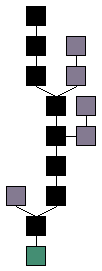
\includegraphics[scale=1]{blockchain.png}
\caption{La Blockchain à ses débuts}
\end{center}
\end{figure}

\subsubsection{Structure d'un bloc}

Les blocs de transactions sont créés par les mineurs et ont la structure suivante.

\begin{figure}[H]
\begin{itemize}
\renewcommand{\labelitemi}{$\bullet$}
\renewcommand{\labelitemii}{$\star$}

\item Header:
\begin{itemize}
\item h(bloc précédent)
\item h(Body)
\item timestamp
\item target (nombre)
\item nonce (nombre) 
\item[ ]
\end{itemize}

\item Body:
\begin{itemize}
\item Coinbase $Tx$
\item $Tx1$
\item $Tx2$
\item $\ldots$
\item $Txn$
\end{itemize}

\end{itemize}

\caption{Un bloc de transaction}
\end{figure}

Un mineur souhaitant créer un bloc va donc récupérer des transactions sur le réseau peer-to-peer, vérifier qu'elles sont valides avec la blockchain actuelle et les ajouter dans le body du bloc. Il pointe sur le bloc le plus récent de la blockchain avec h(bloc précédent). Mais pour que son bloc soit valide il doit à présent résoudre un challenge : il doit trouver un nonce tel que $h(Header)<target$. Or le seul moyen de trouver un tel nonce est d'essayer une multitude de nonces possibles à la suite. Cela demande une très grande puissance de calcul. S'il parvient à résoudre ce problème, le mineur peut donc diffuser le bloc, il est rémunéré par une transaction particulière qu'il introduit avant les transactions qu'il récolte. C'est la coinbase transaction. Elle donne 25 btc à l'adresse que le mineur a choisie.

\subsubsection{Règle de lecture de la Blockchain}

Comme on le voit sur la figure 7, il est possible que dans la blockchain plusieurs blocs pointent sur le même bloc. Il y a alors plusieurs branches possibles. La branche qui détermine les transactions valides à un instant t est la branche la plus longue en partant de la racine (la branche en noir sur la figure 7).

\subsection{Compétition entre les mineurs}

La difficulté est réglée pour qu'un bloc soit miné environ toutes les 10 minutes. Dès qu'un nouveau bloc est miné, les mineurs entrent donc en compétition pour miner le prochain bloc. Ils constituent chacun un bloc avec des transactions valides et cherchent à trouver un nonce valide. Le premier qui trouve un nonce valide diffuse son bloc sur le réseau et il est ajouté à la blockchain. Les mineurs sont donc en compétition pour miner les blocs. Le seul moyen pour un mineur d'être payé est d'intégrer un bloc qu'il a miné dans la blockchain. Autrement toutes ses dépenses (matériels informatiques de calcul rapide, électricité, ...) sont faites à perte.

\subsubsection{Hashrate}

On appelle hashrate le nombre de tentative de nonce que peut faire un mineur en une seconde. Plus son hashrate est élevé plus un mineur a de chances de miner un bloc. Plus précisément, à chaque seconde la probabilité pour un mineur de miner un bloc est égale au ratio de son hashrate sur le hashrate total (ie le hasrate cumulé de tous les mineurs).

\subsubsection{Fork}

On parle de fork lorsque dans la blockchain deux branches partent du même bloc. Sur la figure 7 il y a plusieurs fork. Une fork peut se produire par exemple lorsque deux mineurs minent un bloc à peu près en même temps. La probabilité est assez faible mais cela arrive de temps en temps. Cela crée donc deux branches. Une partie des mineurs va décider de miner sur la branche 1 (donc ils cherchent un bloc qui pointe sur cette branche) et l'autre partie va décider de miner sur la branche 2. Supposons par exemple que le hashrate soit plus important sur la branche 1. La branche 1 va donc avancer plus vite que le branche 2, et comme le hashrate de la branche 1 est supérieur il est certain qu'elle finira forcément par être plus longue que la branche 2. Il est donc peu rentable de miner des blocs sur la branche 2 puisque ceux-ci ne seront sûrement jamais dans la branche principale de la blockchain. C'est pourquoi très vite les mineurs de la branche 2 vont basculer sur la branche 1. La branche 2 va donc être abandonnée.

\subsubsection{Attaque des $51\%$}

Si un mineur possède plus de $51\%$ du hashrate total il peut alors décider de créer un branche qui part de n'importe où dans la blockchain et miner dessus jusqu'à ce que cette branche devienne la plus longue. Comme il possède plus de la moitié du hashrate total il est certain que cette branche finira par devenir la plus longue. Ce mineur peut donc réécrire l'historique des transactions comme il l'entend. Dans ce cas là Bitcoin devient centralisé et c'est ce mineur qui décide quelles transactions sont acceptées ou non, avec possibilité de revenir en arrière. Il est tout puissant. Cela signifie donc la mort de Bitcoin.


\subsection{Impossibilité du double-spend}

Un des buts principaux de la blockchain est que le double-spend soit impossible. Prenons un exemple, il y a dans la blockchain une transaction $Tx$ qui donne 1 btc à l'adresse $adr_B$ de Bob. Bob va essayer d'utiliser deux fois cet output. Il crée donc les transactions $Tx1$ et $Tx2$ suivantes :

\begin{figure}[H]
\begin{itemize}
\renewcommand{\labelitemi}{$\bullet$}
\renewcommand{\labelitemii}{$\star$}

\item Input
\begin{itemize}
\item $h(Tx)$
\item $K_{Pub}^{B}$
\item[$\bullet$] $signature(K_{Pri}^{B}, Tx1^*)$
\end{itemize}

\item Output
\begin{itemize}
\item value : 1 btc
\item $adr_A$
\end{itemize}

\end{itemize}

\caption{Transaction $Tx1$}
\end{figure}



\begin{figure}[H]
\begin{itemize}
\renewcommand{\labelitemi}{$\bullet$}
\renewcommand{\labelitemii}{$\star$}

\item Input
\begin{itemize}
\item $h(Tx)$
\item $K_{Pub}^{B}$
\item[$\bullet$] $signature(K_{Pri}^{B}, Tx2^*)$
\end{itemize}

\item Output
\begin{itemize}
\item value : 1 btc
\item $adr_E$
\end{itemize}

\end{itemize}

\caption{Transaction $Tx2$}
\end{figure}

La transaction $Tx1$ envoie 1 btc à l'adresse de Alice et la transaction $Tx2$ 1 btc à l'adresse d'Eve. Bob diffuse ces deux transactions sur le réseau. Chacune des transaction est valide séparément cependant elles ne peuvent pas être valides en même temps car elle utilisent le même output. Elles ne peuvent donc pas se trouver dans le même bloc ou dans la même branche. Par conséquent les mineurs qui essaient de miner un nouveau bloc vont intégrer dans leur bloc soit $Tx1$ soit $Tx2$ mais pas les deux à la fois. Si le premier bloc à être miné contient $Tx1$ par exemple alors $Tx2$ ne pourra jamais être intégré dans cette branche. Cependant $Tx2$ peut-être intégrée dans une branche parallèle et si cette branche parallèle devient plus longue que la branche de $Tx1$ c'est $Tx2$ qui deviendra valide. Cependant si l'écart entre la branche de $Tx1$ et la plus longue des branches parallèles est plus grand que 6 blocs par exemple alors il est très peu probable que la branche de $Tx1$ soit rattrapée. $Tx1$ restera donc valide, et $Tx2$ non valide. Par conséquent si Alice et Eve attendent assez longtemps (de l'ordre de 6 blocs par exemple) elles sauront pratiquement à coup sûr quelle transaction est valide. Le double-spend n'est donc pas possible du moment que l'on attend quelques blocs avant de considérer un paiement comme valide.

\section{Au delà des principes du protocole}
\subsection{Mise en \oe{}uvre du protocole et découpage des fonctions}
Avec ce qu'on a vu auparavant, on peut déclarer que le protocole Bitcoin est sûr pourvu que :\begin{itemize}
	\item les clefs secrètes restent secrètes
	\item on a accès au consensus atteint par le réseau, c'est-à-dire à la \textit{blockchain}\\
\end{itemize}
Tout d'abord, il convient de noter que l'accès à la \textit{blockchain} est un processus assez lourd : actuellement (avril 2015), l'ensemble de la \textit{blockchain} représente 30 Go ; de plus, par construction un nouveau bloc est ajouté toutes les 10 minutes environ, ce qui suppose une connexion permanente, et des calculs fréquents pour déterminer la validité d'un nouveau bloc. On voit que cette vision extensive de la \textit{blockchain} est difficilement compatible avec les capacités par exemple d'un téléphone portable, alors que c'est assez précisément en étant implémenté sur ce type d'appareil que Bitcoin pourrait remplacer nos moyens de paiement actuels.\\\\ 
De plus, les deux conditions indiquées ci-dessus sont malheureusement assez antagonistes : l'accès à la \textit{blockchain} suppose une connectivité avec l'extérieur, ce qui est nécessairement un facteur de risque pour la sécurité des clefs.\\\\
Cependant, l'architecture de Bitcoin rend possible de séparer les différentes fonctions d'un portefeuille, et en particulier d'isoler la partie signature. De façon intéressante, cette séparation peut même se faire entre différents acteurs, le détenteur d'une adresse délégant une partie de l'ensemble des fonctions d'un portefeuille Bitcoin à une autre entité.\\\\
Dans cette section, nous exposons les différents types de clients Bitcoin qui existent à ce jour (en nous référant à des implémentations existantes) et proposons une première analyse de leurs avantages (en termes de simplicité ou de légèreté) et des changements, en bien ou en mal, qu'ils induisent en termes de sécurité. Pour présenter ces différents types de clients, nous partons des deux conditions évoquées plus haut, qui se traduisent en deux fonctions que le protocole Bitcoin offre : \begin{itemize}
	\item vérifier la réception d'une transaction
	\item émettre un paiement
\end{itemize}
Finalement, nous présentons aussi les \textit{thin clients}, qui sont à l'origine des incidents qui ont semblé atteindre Bitcoin mais dont nous verrons que la sécurité est totalement orthogonale au protocole lui-même. 
\subsection{Vérifier la réception d'une transaction : blockchain et sécurité}
Comme nous l'avons évoqué, l'ensemble de la \textit{blockchain} peut être trop lourd pour des appareils sur lesquels il serait pourtant souhaitable de pouvoir utiliser Bitcoin. Nous présentons tout d'abord le \textit{design} initial et une optimisation, puis les attaques auxquelles les deux sont vulnérables.
\subsubsection{Full clients}
\begin{figure}[h]
	\centering
	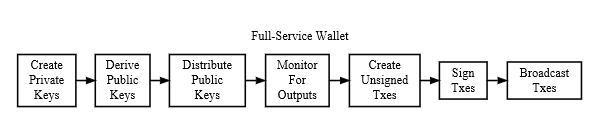
\includegraphics[width=10cm]{en-wallets-full-service}
\end{figure}
Ce genre de clients implémente la totalité du protocole Bitcoin -le client original est d'ailleurs de ce type - et garde en mémoire une copie de la totalité de la \textit{blockchain}. Leurs fonctionnalités peuvent se diviser en deux parties :
\begin{itemize}
	\item \textit{publique}\begin{itemize}
		\item découvrir d'autres n\oe{}uds et communiquer avec eux
		\item envoyer et recevoir des transactions et des blocs
		\item enregistrer tous les blocs valides
		\item vérifier toutes les transactions reçues et \textit{broadcaster} toutes celles qui sont valides
	\end{itemize}
	\item \textit{pour l'utilisateur} \begin{itemize}
		\item stocker son historique de transactions (et les clefs privées pour le "portefeuille")
		\item offrir une interface (GUI ou ligne de commande) pour afficher les avoirs et l'historique des transactions (et générer de nouvelles transactions)\\
	\end{itemize}
\end{itemize}
La partie sur les clefs privées n'est pas celle qui nous intéresse ici : concernant notre axe, \textit{vérifier la réception d'une transaction}, on voit que ce type de client, qui a accès à toutes les transactions, peut en particulier avoir accès à celles à destination de l'utilisateur. C'est le type de client qui offre l'accès le plus complet à la \textit{blockchain} et donc aux transactions reçues.\\\\
Ces clients renforcent la solidité du réseau et le rendent moins vulnérable aux attaques, mais sont coûteux en termes de mémoire, d'opérations (ils vérifient la validité de transactions qui ne concernent pas l'utilisateur) et de frais liés au réseau (ils reçoivent et émettent des transactions et des blocs en permanence).
\subsubsection{Headers-only clients}
Pour les appareils limités en mémoire, ou selon la volonté de l'utilisateur, un deuxième type de client existe, qui ne garde pas en mémoire toute la \textit{blockchain} mais uniquement les \textit{headers} des blocs (ce qui en mai 2012 représentait 14 Mo, à comparer avec les 2 Go de la totalité de la chaîne à la même période). Ils ne téléchargent la totalité d'un bloc que s'ils attendent une transaction, ou s'ils cherchent dans l'ensemble de la chaîne des transactions liées à des clefs qu'ils détiennent. Pour vérifier la validité d'une transaction les concernant, les n\oe{}uds utilisant ce client allégé se reposent sur la procédure \textit{Simplified Payment Verification}, décrite dès le papier fondateur. Dans la suite, nous décrivons le modèle utilisé par \textit{bitcoinj}.\\\\
Cette procédure simplifiée repose sur les n\oe{}uds mettant en \oe{}uvre la totalité du protocole (i.e. ayant en mémoire la totalité de la chaîne), auxquels on délègue la surveillance de la totalité de la \textit{blockchain}. Si le client bitcoinj se connecte à l'un d'entre eux, il ne sera informé d'une transaction que si celle-ci est jugée valide par ce n\oe{}ud. Une fois cette transaction incorporée dans un nouveau bloc (ce que le client bitcoinj peut vérifier s'il récupère ce bloc et contrôle sa validité), la profondeur de cette transaction dans la chaîne passe à 1, et le client bitcoinj ne récupère plus que les \textit{headers} des blocs suivants (qui à chaque fois contiennent une référence au bloc précédent), augmentant à chaque fois la profondeur de la transaction qui l'intéresse de 1. Il considère la transaction comme sûre une fois qu'elle est à une profondeur suffisante dans la chaîne (la valeur typiquement retenue étant de 6), c'est à dire une fois qu'il estime suffisamment peu probable que cette branche de la chaîne ne soit pas la branche finalement retenue.\\\\
On voit ici que l'on fait confiance à un tiers pour nous signaler une transaction nous concernant. Du point de vue de la sécurité, cela peut permettre à un n\oe{}ud malicieux de nous cacher une transaction qui se situe dans la \textit{blockchain} (mais cette situation est temporaire, elle cessera dès la connexion à un n\oe{}ud honnête), mais en aucun cas de nous faire croire que l'on a reçu une transaction qui n'a en réalité pas été validée (puisque l'on peut contrôler la validité des blocs que l'on récupère), ce qui serait plus gênant\footnote{Si on fournissait une contrepartie à cette transaction fictive,...}. La sécurité de ce type de client est donc globalement similaire à celle des \textit{full clients}, si ce n'est qu'il est plus facile de cacher temporairement une transaction bien réelle à ce type de client.
\subsubsection{Attaques sur la \textit{blockchain}}
Les deux types de clients évoqués ci-dessus sont susceptibles de subir des attaques temporaires sur la perception qu'ils ont de la \textit{blockchain}, ou plus précisément de la branche valide de la \textit{blockchain}, et ainsi de considérer comme validées des transactions qui \textit{in fine} ne feront pas partie de la \textit{blockchain}.\\\\
L'attaque la plus "simple", appelée \textit{Sybil attack}, a lieu si l'attaquant a la possibilité de contrôler entièrement notre connexion à Internet, et ainsi (1) de nous présenter un faux réseau dans lequel tous les n\oe{}uds acceptent cette transaction pour nous faire croire qu'elle est valide, puis (2) d'ajouter des blocs au-dessus pour nous faire croire qu'elle est définitive. \\\\
Une attaque plus subtile, appelée \textit{timestamp attack}, repose d'une part sur les valeurs arrêtées dans le protocole à propos de la fenêtre temporelle qu'un client considère pour considérer des blocs comme valides\footnote{Pour rappel, la difficulté du minage est ajustée pour qu'un nouveau bloc soit miné toutes les 10 minutes en moyenne} et d'autre part sur le fait que pour éviter des dérives d'horloge qui entraîneraient des problèmes du fait de cette notion de fenêtre temporelle, les clients n'utilisent pas le temps système de la machine sur laquelle ils sont installés mais une moyenne des temps indiqués par leurs pairs du réseau Bitcoin. En créant des pairs fictifs qui interagissent avec le client Bitcoin de la cible, un attaquant peut faire dériver son horloge jusqu'à un point où ce client ciblé n'acceptera plus les blocs minés par le vrai réseau\footnote{avec lequel il est toujours en contact, contrairement à l'attaque précédente où il était totalement isolé} ; l'attaquant a ainsi le temps de proposer à la cible une branche de la \textit{blockchain} qu'il mine tout seul et dans laquelle il met ce qu'il veut ; la cible fournit en échange des transactions qu'elle croit validées le bien ou service correspondant, et ne se rend compte de la supercherie que quand son horloge revient vers le temps réel du réseau et qu'elle constate la réalité de la \textit{blockchain}, c'est à dire que la branche qu'elle considérait comme étant la plus longue est en fait plus courte que la branche légitime et n'est donc pas celle qui sera retenue par le réseau.\\\\
Pour contrecarrer ces deux attaques, une possibilité serait de mettre en place des clients qui mesurent la vitesse à laquelle de nouveaux blocs sont minés : en effet, dans le cas où l'attaquant n'est pas dans une configuration de puissance de type 51\%, cette vitesse décroîtrait brutalement avec l'usurpation, et le client pourrait ainsi signaler à l'utilisateur que la situation est douteuse et qu'il ferait mieux de se méfier. Ce n'est toutefois pas une réponse certaine et définitive.
\subsection{Emettre des paiements : sécurité des clefs}
Comme nous l'avons évoqué, l'ouverture permanente de notre système vers l'extérieur afin de participer pleinement au protocole Bitcoin ou même simplement de vérifier la réception de paiements sur des adresses en particulier semble difficilement conciliable avec la sécurité des clefs privées qui permettent de dépenser les bitcoins : les bonnes pratiques habituelles de la sécurité enjoignent à isoler autant que faire se peut les informations qui ne doivent absolument pas être compromises.
\subsubsection{La sécurité des clefs dans les \textit{full} et \textit{headers-only clients}}
La sécurité initiale des clients Bitcoin où les fonctions de réception et d'émission des paiements sont sur le même appareil repose sur l'encryption des clefs privées, au moyen de l'algorithme AES-256-CBC et d'un mot de passe. Au moment de la création d'une clef privée, une \textit{master key} aléatoire est générée, qui sert à crypter la clef privée ; la \textit{master key} est elle-même cryptée au moyen d'un mot de passe (à partir duquel une clef est générée à travers plusieurs tours\footnote{Le nombre de tours est adapté au CPU de l'appareil sur lequel est effectuée la création de la clef privée} de la fonction SHA 512).\\\\
Ce mécanisme a pour but de ralentir une attaque de type force brute pour décrypter les clefs sur le disque. Cependant, il est inopérant contre des logiciels de type \textit{key logger}.\\\\
Les deux types de clients suivants ont pour objectif de réduire le risque de compromission du stockage des clefs.
\subsubsection{Watch-only / sign-only clients}
\paragraph{Watch-only clients}
Ce type de client se consacre uniquement à la vérification des transactions : il est conçu par exemple pour des commerçants, qui fournissent un produit ou un service après vérification de la réception d'une transaction ; cette vérification se fait typiquement sur un ordinateur situé dans un lieu accessible au public (café,... sur lequel un client malveillant pourrait par exemple brancher une clef USB) ou sur un serveur en ligne.\\\\
L'idée est que ce client ne dispose que des clefs publiques associées aux adresses dont il veut vérifier qu'elles ont bien reçu un paiement. Il peut ainsi être connecté à l'extérieur et vérifier l'état de la \textit{blockchain} ; en cas de compromission, l'attaquant pourra accéder à l'historique des transactions reçues mais en aucun cas dépenser les bitcoins correspondants, puisqu'il est virtuellement impossible de remonter aux clefs privées à partir des clefs publiques.
\paragraph{Sign-only client}
Ce type de client est dual du précédent : il se consacre uniquement à la signature de transactions.
Les \textit{signing-only clients} vont encore une étape plus loin que les \textit{headers-only clients} dans la délégation de compétence : le client ne télécharge pas la blockchain, ni même les headers. Il se base sur un autre client pour lui fournir les transactions qui concernent l'utilisateur et la situation financière de ce dernier, et ne garde en propre que la partie signature.
\begin{figure}[h]
	\centering
	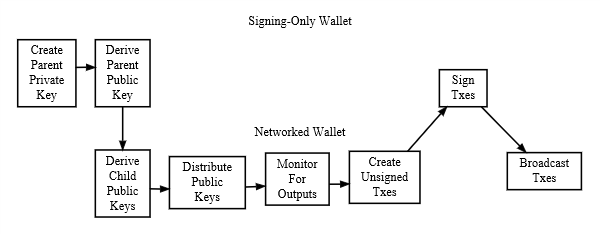
\includegraphics[width=10cm]{en-wallets-signing-only}
\end{figure}
 \\Ce cas de figure a deux fonctions principales :\begin{itemize}
	\item sécuriser les clefs : un utilisateur peut être prêt à installer sur un de ses appareils un client Bitcoin complet, mais estimer que conserver ses clefs sur un appareil connecté à l'extérieur n'est pas raisonnable ; il découpe ainsi son client en deux parties, l'une participant au réseau et lui indiquant notamment les transactions qu'il reçoit, vérifiant leur validité et leur inclusion dans la chaîne,... et l'autre, sur un appareil distinct et isolé de l'extérieur, contenant ses clefs privées et étant donc la seule à pouvoir dépenser ses bitcoins. Il y a plusieurs possibilités pour implémenter cette séparation :\begin{itemize}
		\item Faire des transferts avec par exemple une clef USB entre les deux équipements, ce qui est contraignant
		\item Acheter une implémentation physique de cette partie signature, par exemple un appareil doté d'une connexion USB, sur lequel peut se trouver un dispositif de type code PIN,... pour plus de sécurité. Cette situation est dénotée sous le terme \textbf{hardware wallet}.
	\end{itemize}
	\item alléger le protocole Bitcoin, pour un usage mobile par exemple, en confiant à un serveur le soin de suivre les transactions nous concernant et de nous indiquer nos avoirs. Il y a alors deux cas de figure : \begin{itemize}
		\item si ce serveur est géré par quelqu'un d'autre, cela suppose un certain niveau de confiance puisque le serveur peut nous induire en erreur en nous indiquant de fausses transactions que l'on aurait reçues, nous trompant ainsi sur la quantité de bitcoins que nous détenons. Ce genre d'attaque est d'une importance limitée, puisque le serveur ne peut en aucun cas dépenser lui-même les bitcoins que nous possédons (nous faire signer des transactions contre notre volonté). Il est de plus possible d'éviter cette attaque en nous connectant à plusieurs serveurs indépendants
		\item on se connecte à notre propre serveur\footnote{Il existe des logiciels open source permettant de réaliser ce genre de serveurs}. L'intérêt de cette démarche est de pouvoir implémenter un \textit{full client} de manière distribuée : la partie signature sur un appareil contraint (type mobile), et en appui un serveur externe pour réaliser la partie la plus exigeante en termes de calculs et de connexions.
	\end{itemize}
	\item Dans tous les cas, le client peut être une application PC, mobile ou web ; dans le cas d'une application Web, la signature est faite dans le browser, et les clefs ne sont donc pas envoyées. 
\end{itemize}

\subsection{Thin clients}
Ces clients sont ceux dont les failles ont rencontré un large écho dans la presse : Mt.Gox,... Ils vont une étape plus loin dans la délégation par apport aux \textit{sign-only} clients, mais c'est précisément cette étape qui va à l'encontre des principes mêmes de Bitcoin et transforme totalement l'analyse de la sécurité - du point de vue du détenteur des bitcoins.\\\\
Le client ne détient pas ses clefs et ne signe pas lui-même ses transactions, il demande à un serveur distant de faire cela pour lui ; il se connecte à ce serveur distant avec une sécurité de type login-mot de passe. Cela implique une confiance certaine en l'administrateur du serveur, qui détient effectivement les clefs, et en la sécurité d'une installation que l'on ne contrôle pas face aux attaques classiques concernant des sites Internets, des serveurs,...; dans tous les cas la sécurité devient largement décorrélée du protocole Bitcoin lui-même.\\\\ En un sens, c'est exactement la même chose qu'une banque et toute la motivation de base du Bitcoin - se passer de tiers-partie - disparaît. Il convient aussi de souligner que les acteurs de l'écosystème Bitcoin sont loin du niveau de garantie offert par les banques, ne serait-ce que du fait de l'absence de réglementation.

\bibliography{biblio}{}
\bibliographystyle{plain}

\end{document}